\documentclass{beamer}
\usepackage[utf8]{inputenc}
\usepackage[T1]{fontenc}
\usepackage{bookmark}
\usetheme{Madrid}
\usetheme{default}
\usecolortheme{beaver}
\usepackage{graphicx}
\graphicspath{ {pics} }
\usepackage{amsmath}
\usepackage{amssymb}
\usepackage{framed}
\usepackage{tikz}
\usepackage[]{xcolor}
\usepackage[most]{tcolorbox}
\usepackage{pgfplots}
\pgfplotsset{compat=1.18}
\usepackage{booktabs}
\usepackage{tabularx} % Added tabularx package for better table width control

\title{What is Learning?}
\author{}
\date{}

\begin{document}

\frame{\titlepage}

\begin{frame}{What is  Learning ?}
    \begin{itemize}
        \item Learning is the process of converting experience into expertise or knowledge.
        \item Training data represents experience.
        \item The output of learning is expertise, often in the form of a computer program.
        \item Key questions in learning:
        \begin{itemize}
            \item What is the training data?
            \item How can learning be automated?
            \item How do we evaluate learning success?
        \end{itemize}
    \end{itemize}
\end{frame}

\begin{frame}{What is Reasoning?}
    \begin{itemize}
        \item Reasoning is the ability to draw logical conclusions from known facts or learned knowledge.
        \item It does not require large amounts of data but rather depends on logical inference.
    \end{itemize}
\end{frame}


\begin{frame}{Example: Animal Learning}
    \textbf{Bait Shyness in Rats}
    \begin{itemize}
        \item Rats sample novel food cautiously.
        \item If the food causes illness, they avoid it in the future.
        \item Past experience informs future decisions.
    \end{itemize}
\end{frame}

\begin{frame}{Example: Machine Learning Task}
    \textbf{Spam Email Filtering}
    \begin{itemize}
        \item Naive approach: Memorization of past spam emails.
        \item Limitation: Cannot classify unseen emails.
        \item Solution: \textbf{Generalization using inductive reasoning}.
        \item Like rats apply their attitude to new unseen examples of food with similar smell and taste
        \item Extract patterns (e.g., words indicating spam) to classify new emails.
    \end{itemize}
\end{frame}

\begin{frame}{Types of Reasoning in AI and ML}
    \textbf{1. Inductive Reasoning (Primary)}
    \begin{itemize}
        \item Extracts patterns from observed data to make predictions.
        \item Used in deep learning and LLMs.
        \item \textbf{Example:} A spam classifier learns from previously labeled emails and generalizes patterns to detect new spam messages.
    \end{itemize}

    \textbf{2. Abductive Reasoning (Inference to Best Explanation)}
    \begin{itemize}
        \item Guesses the most probable explanation given incomplete data.\@
        \item Used in medical diagnosis and troubleshooting AI.\@
        \item \textbf{Example:} A doctor observes symptoms like fever and cough and infers that the patient likely has the flu, even without a lab test.
    \end{itemize}

    \textbf{3. Analogical Reasoning (Pattern Transfer)}
    \begin{itemize}
        \item Applies knowledge from one context to another.
        \item Used in AI-powered tutoring and cross-domain learning.
        \item \textbf{Example:} AI that learns human speech patterns in English and transfers that learning to generate speech in another language.
    \end{itemize}
\end{frame}

\begin{frame}{Probabilistic and Other Reasoning Types (Part 1)}
    \textbf{4. Bayesian Reasoning (Probabilistic Prediction)}
    \begin{itemize}
        \item Uses probability to predict outcomes.
        \item Used in spam filtering and AI language models.
        \item \textbf{Example:} A Bayesian spam filter assigns probabilities to words appearing in spam emails and calculates the likelihood that a new email is spam.
    \end{itemize}

    \textbf{5. Deductive Reasoning (Not Used in LLMs)}
    \begin{itemize}
        \item Moves from general rules to specific conclusions.
        \item LLMs lack strict logical reasoning.
        \item \textbf{Example:} In mathematics, if all squares have four sides and a shape is a square, it must have four sides.
    \end{itemize}
\end{frame}

\begin{frame}{Probabilistic and Other Reasoning Types (Part 2)}
    \textbf{6. Causal Reasoning (Understanding Cause-and-Effect)}
    \begin{itemize}
        \item Determines causal relationships rather than correlations.
        \item LLMs struggle with causality.
        \item \textbf{Example:} In healthcare, researchers identify that smoking causes lung cancer, rather than just observing that smokers have higher cancer rates.
    \end{itemize}

    \textbf{7. Counterfactual Reasoning (What-If Thinking)}
    \begin{itemize}
        \item Explores hypothetical scenarios.
        \item Used in risk analysis and AI decision-making.
        \item \textbf{Example:} A self-driving car AI simulates different driving scenarios to decide the safest course of action in an emergency.
    \end{itemize}
\end{frame}


\begin{frame}{Limitations of Inductive Reasoning}
    \textbf{Pigeon Superstition Experiment (B.F. Skinner)}
    \begin{figure}
        \centering
        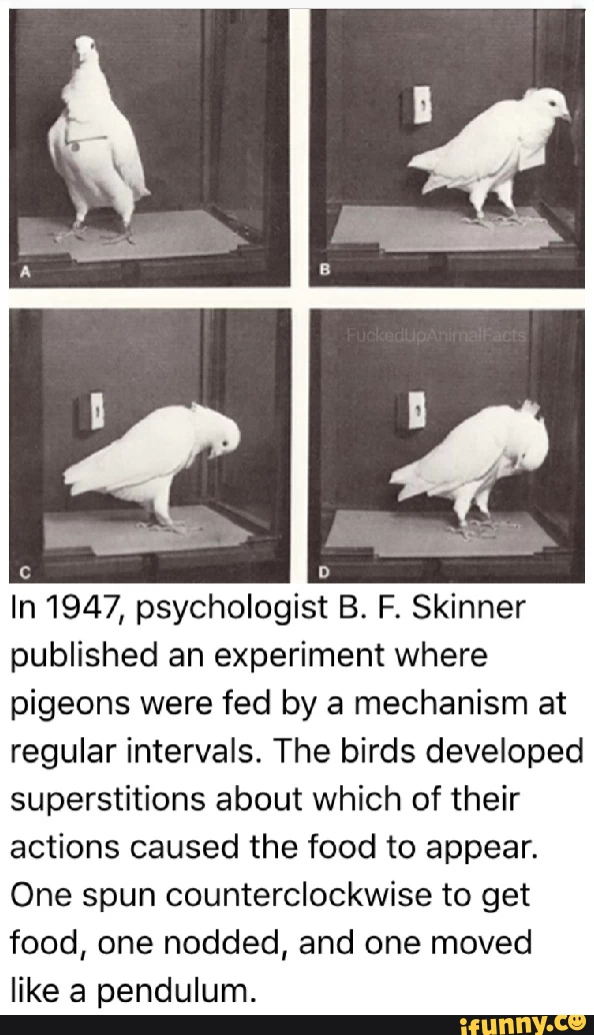
\includegraphics[width=0.3\textwidth]{figures/superstition.png}
    \end{figure}
\end{frame}

\begin{frame}{Bait Shyness Revisited: Garcia \& Koelling Experiment (1966)}
    \begin{itemize}
        \item The experiment was conducted by John Garcia and Robert Koelling to study \textbf{selective associative learning} in rats.
        \item It demonstrated that \textbf{not all stimuli are equally associated} with consequences, challenging traditional learning theories.
        \item The experiment used a \textbf{compound stimulus} consisting of:
        \begin{itemize}
            \item A \textbf{taste cue} (saccharin-flavored water).
            \item \textbf{Audiovisual cues} (lights and sounds that played while drinking).
        \end{itemize}
        \item After exposure to the stimuli, the rats were subjected to an \textbf{aversive event}:
        \begin{itemize}
            \item \textbf{Group 1: Induced Illness} (nausea caused by mild radiation or a toxin).
            \item \textbf{Group 2: Electric Shock} (mild foot shocks upon drinking).
        \end{itemize}
    \end{itemize}
\end{frame}

\begin{frame}{Key Findings of Garcia \& Koelling Experiment }
    \begin{itemize}
        \item \textbf{Illness-Induced Group:}
        \begin{itemize}
            \item Developed a \textbf{strong aversion} to the \textbf{taste cue} (saccharin water).
            \item Showed little to no aversion to \textbf{audiovisual cues} (lights and sounds).
        \end{itemize}
        \item \textbf{Shock-Induced Group:}
        \begin{itemize}
            \item Developed a \textbf{strong aversion} to \textbf{audiovisual cues} (lights and sounds).
            \item Showed no aversion to \textbf{taste cue} (saccharin water).
        \end{itemize}
    \end{itemize}
\end{frame}

\begin{frame}{Key Findings of Garcia \& Koelling Experiment }
    \begin{itemize}
        \item This demonstrated that rats were \textbf{biologically predisposed to associate taste with internal discomfort (nausea)} and \textbf{sounds/lights with external discomfort (shock)}.
    \end{itemize}
\end{frame}

\begin{frame}{Key Findings of Garcia \& Koelling Experiment}
    \begin{itemize}
        \item Bait shyness learning in rats incorporates prior knowledge, known as inductive bias.
        \item Rats are biased towards detecting patterns and ignoring other temporal correlations.
        \item Pigeons, however, adopt any explanation for the occurrence of food.
    \end{itemize}
\end{frame}

\begin{frame}{Scientific Implications of the Experiment}
    \begin{itemize}
        \item The experiment \textbf{challenged the traditional idea of equipotentiality}, which assumed that any stimulus can be associated with any consequence.
        \item It provided evidence that \textbf{evolution influences learning mechanisms}.
        \item Animals (including humans) have \textbf{prewired biases} for learning certain associations based on survival advantages.
        \item \textbf{Biological Constraints on Learning:}
        \begin{itemize}
            \item Taste is more likely to be linked with food poisoning.
            \item Sounds or visual cues are more likely to be linked with external dangers (e.g., predators, electric shocks).
        \end{itemize}
    \end{itemize}
\end{frame}

\begin{frame}{Key Takeaways from the Garcia \& Koelling (1966) Experiment}
    \begin{itemize}
        \item Learning is not arbitrary – it requires \textbf{inductive bias}.
        \item Not all features are equally useful for learning.\@
        \item Correlation does not imply causation.
    \end{itemize}
\end{frame}

\begin{frame}{Key Takeaways from the Garcia \& Koelling (1966) Experiment}
    \begin{itemize}
        \item Evolutionary constraints shape learning – \textbf{domain knowledge matters}.
        \item The No-Free-Lunch theorem – \textbf{There’s no universal learner}.
        \item The role of evolutionary and pre-trained knowledge in AI.
    \end{itemize}
\end{frame}



\section{Inductive Bias in Machine Learning}

\begin{frame}{What is Inductive Bias?}
    \textbf{Definition:}
    \begin{itemize}
        \item Inductive bias refers to the set of assumptions that a learning algorithm makes to generalize from limited training data to unseen data.
        \item Since real-world data is often incomplete or noisy, a model must rely on prior knowledge or constraints to make meaningful predictions.
    \end{itemize}

    \textbf{Why is Inductive Bias Important?}
    \begin{itemize}
        \item Machine learning models do not have infinite training data.
        \item They must generalize from past observations to unseen cases.
        \item Without a bias, a model may overfit (memorize data without true learning).
    \end{itemize}
\end{frame}

\subsection{Types of Inductive Biases}

\begin{frame}{Types of Inductive Biases}
    \textbf{1. Preference for Simpler Models (Occam’s Razor)}
    \begin{itemize}
        \item \textbf{Assumption:} Simpler explanations are preferred over complex ones.
        \item \textbf{Example:} Decision trees with fewer splits are preferred because they generalize better.
        \item \textbf{In Deep Learning:} Regularization techniques (L1, L2) penalize complex models to enforce simplicity.
    \end{itemize}
\end{frame} 

\begin{frame}{Types of Inductive Biases}
    \textbf{2. Smoothness Assumption}
    \begin{itemize}
        \item \textbf{Assumption:} Data points that are close together should have similar outputs.
        \item \textbf{Example:} In image classification, two similar images should belong to the same class.
        \item \textbf{In ML:} K-Nearest Neighbors (KNN) assumes that nearby data points have the same label.
    \end{itemize}
\end{frame} 

\begin{frame}{Types of Inductive Biases}
    \textbf{3. Similar Features Should Have Similar Effects}
    \begin{itemize}
        \item \textbf{Assumption:} If two features (e.g., temperature \& humidity) are related, their effects should be similar.
        \item \textbf{Example:} In linear regression, correlated features often have similar coefficients.
        \item \textbf{In ML:}  In decision trees and feature selection algorithms, correlated features (e.g., “annual income” \& “monthly salary”) often contribute similarly to predictions.
    \end{itemize}

\end{frame} 

\begin{frame}{Types of Inductive Biases}

    \textbf{4. Prior Knowledge About the Task (Domain-Specific Bias)}
    \begin{itemize}
        \item \textbf{Assumption:} Certain relationships are more likely in specific tasks.
        \item \textbf{Example:} In natural language processing (NLP), word order matters (e.g., “The cat sat on the mat” is not equal to “The mat sat on the cat”).
        \item \textbf{In ML:} Transformers (e.g., BERT, GPT) use positional embeddings to capture sentence structure.
    \end{itemize}
\end{frame}

\begin{frame}{Types of Inductive Biases}
\textbf{5. Invariance Bias (Translation, Rotation, Scale Invariance)}
    \begin{itemize}
        \item \textbf{Assumption:} Some transformations should not change predictions.
        \item \textbf{Example:} In computer vision, rotating an image of a cat should still classify it as a cat.
        \item \textbf{In ML:} CNNs use convolutional filters to enforce translation invariance.
    \end{itemize}
\end{frame} 

\begin{frame}{Types of Inductive Biases}
    \textbf{6. Sparsity Assumption}
    \begin{itemize}
        \item \textbf{Assumption:} Only a few features are truly important.
        \item \textbf{Example:} In text classification, most words are irrelevant, and only a few indicate spam.
        \item \textbf{In ML:} L1 regularization forces models to select only the most important features.
    \end{itemize}
\end{frame}

\begin{frame}{Inductive Bias in Machine Learning Models}
    \textbf{Example 1: Human Learning vs. ML}
    \begin{itemize}
        \item \textbf{Humans:} When a child learns what a “dog” is, they assume all dogs have four legs, fur, and bark. This is an inductive bias—it helps the child generalize.
        \item \textbf{ML Model:} If trained on 100 pictures of dogs, an image classifier may learn that four legs + fur are key features of a dog. However, without bias, it may fail when seeing a three-legged dog.
    \end{itemize}
\end{frame}


\begin{frame}{Inductive Bias in Convolutional Neural Networks (CNNs)}
    \textbf{CNNs are designed for image processing and rely on three key inductive biases:}
    
    \textbf{1.1 Locality Bias (Local Connectivity)}
    \begin{itemize}
        \item \textbf{Assumption:} Nearby pixels in an image are more relevant to each other than distant pixels.
        \item \textbf{Why it helps?} Instead of treating each pixel separately, CNNs focus on small local features (edges, textures, shapes) before forming high-level representations.
        \item \textbf{Example:} In facial recognition, a CNN first detects eyes, nose, and mouth individually before recognizing an entire face.
    \end{itemize}
\end{frame}
\begin{frame}{Inductive Bias in Convolutional Neural Networks (CNNs)}
    \textbf{1.2 Translation Invariance}
    \begin{itemize}
        \item \textbf{Assumption:} An object in an image should be recognized regardless of its position.
        \item \textbf{Why it helps?} A cat in the top-left corner should be classified as a cat, just as a cat in the bottom-right corner.
        \item \textbf{How it works?} CNNs use shared convolutional filters to detect patterns anywhere in the image.
        \item \textbf{Example:} A handwritten digit “3” should be recognized no matter where it appears in the image.
    \end{itemize}
\end{frame} 

\begin{frame}{Inductive Bias in Convolutional Neural Networks (CNNs)}
    
    \textbf{1.3 Hierarchical Feature Learning}
    \begin{itemize}
        \item \textbf{Assumption:} Complex patterns can be learned by stacking multiple layers of abstraction.
        \item \textbf{Why it helps?} Lower layers detect edges, middle layers detect shapes, and deeper layers detect objects.
        \item \textbf{Example:} A CNN learns small textures → eyes/mouth → full face in image classification.
    \end{itemize}
    
    \textbf{\textit{Takeaway}} CNNs perform better than traditional dense networks for image tasks because of these biases.
\end{frame}

\subsection{Inductive Bias in Recurrent Neural Networks (RNNs and LSTMs)}

\begin{frame}{Inductive Bias in Recurrent Neural Networks (RNNs \& LSTMs)}
    \textbf{RNNs are designed for sequential data (e.g., speech, text, time-series forecasting) and rely on two main biases:}
    
    \textbf{2.1 Temporal Dependency Bias}
    \begin{itemize}
        \item \textbf{Assumption:} Recent information is more important than distant past information.
        \item \textbf{Why it helps?} Words appearing closer together in a sentence are more related.
        \item \textbf{Example:}
        \item In “The cat sat on the mat”, the word “mat” is a likely prediction.
        \item In a time-series forecast, the last few observations are more important.
    \end{itemize}
\end{frame}  
\begin{frame}{Inductive Bias in Recurrent Neural Networks (RNNs \& LSTMs)}
    \textbf{2.2 Order Sensitivity Bias}
    \begin{itemize}
        \item \textbf{Assumption:} The order of input elements matters.
        \item \textbf{Why it helps?} “Dog bites man” is not equal to “Man bites dog.”
        \item \textbf{Example:} Machine translation relies on word ordering to make correct translations.
    \end{itemize}

    \textbf{Takeaway:} RNNs/LSTMs work well for time-dependent problems because they incorporate sequential learning bias.
\end{frame}

\subsection{Inductive Bias in Transformers (e.g., BERT, GPT)}

\begin{frame}{Inductive Bias in Transformers (e.g., BERT, GPT)}
    \textbf{Transformers, which power GPT, BERT, and other large language models (LLMs), incorporate several modern inductive biases that make them highly generalizable:}
    
    \textbf{Attention-Based Bias (Self-Attention)}
    \begin{itemize}
        \item \textbf{Assumption:} Important words in a sentence can be anywhere, not just nearby.
        \item \textbf{Why it helps?} Instead of only relying on adjacent words, transformers attend to relevant words across an entire sentence.
        \item \textbf{Example:}
        \item In “The dog chased the ball across the field, past the trees, over the hill, which was blue.” the word “which” refers to “ball”, even though they are not next to each other.
    \end{itemize}
\end{frame} 

\begin{frame}{Inductive Bias in Transformers (e.g., BERT, GPT)}
    \textbf{Context-Aware Learning Bias}
    \begin{itemize}
        \item \textbf{Assumption:} The meaning of a word depends on its context.
        \item \textbf{Why it helps?} The word “bank” can mean a financial institution or a riverbank, and transformers can disambiguate meaning based on context.
        \item \textbf{Example:}
        \item “I deposited money in the bank” → Financial institution
        \item “The boat was near the river bank” → River side
    \end{itemize}
\end{frame} 

\begin{frame}{Inductive Bias in Transformers (e.g., BERT, GPT)}
    \textbf{3.3 Positional Encoding Bias}
    \begin{itemize}
        \item \textbf{Assumption:} Order still matters, even without RNNs.
        \item \textbf{Why it helps?} Since transformers do not process words sequentially, they use positional encodings to maintain the order of words.
        \item \textbf{Example:}
        \item “She ate an apple” \(\neq\) “An apple ate she.”
    \end{itemize}

    \textbf{\textit{Takeaway:}} Transformers use self-attention, context-awareness, and positional encoding biases, making them more flexible than CNNs and RNNs.
\end{frame}

\begin{frame}{Role of Prior Knowledge in Machine Learning}
    \begin{itemize}
        \item Development of tools for expressing domain expertise, translating it into learning bias and quantifying the effect of such a bias on the success of learning is a central theme of the theory of machine learning
        \item Stronger prior knowledge makes learning from examples easier.
        \item However, stronger prior assumptions reduce the flexibility of learning.
        \item The challenge is to find the right balance between prior knowledge and data-driven learning. 
    \end{itemize}
\end{frame}

\begin{frame}{Key Takeaways}
    \begin{itemize}
        \item Learning involves converting experience into generalizable knowledge.
        \item Different reasoning types play a role in AI and ML
        \item Inductive bias is crucial for generalization and learning efficiency.
        \item Deep learning relies primarily on inductive reasoning.
        \item LLMs approximate abductive and Bayesian reasoning but lack causal and deductive reasoning.
        \item Future AI models may incorporate stronger causal and counterfactual reasoning capabilities.
    \end{itemize}
\end{frame}


\section{Machine Learning}

\begin{frame}{Why Machine Learning}
    \begin{itemize}
        \item For many problems, it’s difficult to program the correct behavior by hand.
        \begin{itemize}
            \item E.g., recognizing objects in images, understanding human speech.
        \end{itemize}
        \item Machine learning approach: program an algorithm to automatically learn from data or experience.
        \item Reasons to use a learning algorithm:
        \begin{itemize}
            \item Hard to code up a solution by hand (e.g., vision, speech).
            \item System needs to adapt to a changing environment (e.g., spam detection).
            \item Want the system to perform better than the human programmers.
            \item Privacy/fairness (e.g., ranking search results).
        \end{itemize}
    \end{itemize}
\end{frame}

\begin{frame}{Machine Learning vs Statistics}
    \begin{itemize}
        \item Both fields try to uncover patterns in data.
        \item Both draw heavily on calculus, probability, and linear algebra, and share many of the same core algorithms.
        \item However, they have different focuses:
        \begin{itemize}
            \item Statistics: Helping scientists and policymakers draw good conclusions.
            \item Machine Learning: Building autonomous agents.
        \end{itemize}
        \item Emphasis differences:
        \begin{itemize}
            \item Statistics: Interpretability and mathematical rigor.
            \item Machine Learning: Predictive performance, scalability, and autonomy.
        \end{itemize}
    \end{itemize}
\end{frame}

\begin{frame}{Relations to AI}
    \begin{itemize}
        \item Nowadays, “machine learning” is often brought up with “artificial intelligence” (AI).
        \item AI does not always imply a learning-based system:
        \begin{itemize}
            \item Symbolic reasoning
            \item Rule-based system
            \item Tree search
            \item etc.
        \end{itemize}
        \item Learning-based system:
        \begin{itemize}
            \item Learned based on the data
            \item More flexibility
            \item Good at solving pattern recognition problems
        \end{itemize}
    \end{itemize}
\end{frame}

\begin{frame}{What is Symbolic AI?}
    \begin{itemize}
        \item Symbolic AI (also known as **Good Old-Fashioned AI, GOFAI**) represents knowledge using **symbols, rules, and logic**.
        \item It uses **explicitly programmed rules** to perform reasoning and problem-solving.
        \item Symbolic AI is based on **formal logic, tree search, and knowledge representation**.
        \item \textbf{Example:} If \textit{All humans are mortal} and \textit{Socrates is human}, then we can deduce that \textit{Socrates is mortal}.
    \end{itemize}
\end{frame}

\begin{frame}{What is Tree Search in Symbolic AI?}
    \begin{itemize}
        \item Tree search is a fundamental approach in Symbolic AI for solving problems by exploring possible states in a **decision tree**.
        \item Algorithms like **Depth-First Search (DFS), Breadth-First Search (BFS), and A* Search** are used to navigate possible solutions.
        \item \textbf{Example:} Chess-playing AI searches possible future board states to decide the best move.
        \item Unlike Machine Learning, tree search does **not generalize from data** but explicitly computes solutions using logical steps.
    \end{itemize}
\end{frame}



\begin{frame}{Rule-Based AI: A Subset of Symbolic AI}
    \begin{itemize}
        \item Rule-Based AI applies Symbolic AI using **explicit if-then rules**.
        \item Rules are manually defined by experts rather than learned from data.
        \item \textbf{Example:} A medical expert system might use rules like:
        \begin{itemize}
            \item IF patient has fever AND cough → Diagnose as flu.
            \item IF transaction amount > \$10,000 → Flag as potential fraud.
        \end{itemize}
        \item Limitation: Rule-based systems **struggle to handle exceptions and uncertain scenarios**.
    \end{itemize}
\end{frame}

\begin{frame}{How Symbolic AI Uses Reasoning}
    \begin{itemize}
        \item Symbolic AI relies on different types of reasoning:
        \begin{itemize}
            \item **Deductive Reasoning:** Uses general rules to reach specific conclusions.
            \item **Inductive Reasoning:** Generalizes from examples.
            \item **Abductive Reasoning:** Chooses the most likely explanation given incomplete information.
            \item **Probabilistic Reasoning:** Uses probabilities to model uncertainty.
        \end{itemize}
        \item Machine Learning models **approximate** these reasoning types but do not explicitly use formal logic.
    \end{itemize}
\end{frame}

\begin{frame}{Limitations of Symbolic AI}
    \begin{itemize}
        \item Difficult to scale—rule-based systems require **manual updates**.
        \item Cannot handle **unstructured data** (e.g., images, speech).
        \item Struggles with **uncertainty**—rules do not adapt to new situations.
        \item Machine Learning **outperforms Symbolic AI** in perception tasks (e.g., NLP, vision).
    \end{itemize}
\end{frame}

\begin{frame}{The Future: Hybrid AI (Neuro-Symbolic AI)}
    \begin{itemize}
        \item **Hybrid AI** combines **Symbolic AI (structured logic)** with **Machine Learning (pattern recognition)**.
        \item **Example:** AI lawyer uses Symbolic AI to interpret legal rules + Machine Learning to analyze past case history.
        \item This approach enhances **explainability, adaptability, and reasoning.**
    \end{itemize}
\end{frame}

\begin{frame}{Final Takeaways}
    \begin{itemize}
        \item \texbf{Symbolic AI} relies on \textbf{explicit rules and logic}.
        \item \textbf{Machine Learning} learns from **data without explicit programming**.
        \item **Rule-Based AI is a subset of Symbolic AI** but lacks flexibility.
        \item Future AI will combine **symbolic reasoning with deep learning** to create **more intelligent and interpretable models**.
    \end{itemize}
\end{frame}

\begin{frame}{Symbolic AI vs Machine Learning}
    \begin{tcolorbox}[colback=white!95!black]
        \begin{tabularx}{\textwidth}{>{\raggedright\arraybackslash\hsize=0.8\hsize}X>{\raggedright\arraybackslash\hsize=1.1\hsize}X>{\raggedright\arraybackslash\hsize=1.1\hsize}X}
            \textbf{Feature} & \textbf{Symbolic AI} & \textbf{Machine Learning} \\
            \midrule
            Knowledge & Rules \& logic & Data \& patterns \\
            \hline
            Interpretability & Explainable & Often a black box \\
            \hline
            Adaptability & Rigid (manual updates) & Can generalize \\
            \hline
            Data Needs & Minimal & Requires large datasets \\
            \hline
            Example Uses & Theorem proving, expert systems & NLP, vision, recommendations \\
        \end{tabularx}
    \end{tcolorbox}
\end{frame}

\end{document}
